\documentclass[1p]{elsarticle_modified}
%\bibliographystyle{elsarticle-num}

%\usepackage[colorlinks]{hyperref}
%\usepackage{abbrmath_seonhwa} %\Abb, \Ascr, \Acal ,\Abf, \Afrak
\usepackage{amsfonts}
\usepackage{amssymb}
\usepackage{amsmath}
\usepackage{amsthm}
\usepackage{scalefnt}
\usepackage{amsbsy}
\usepackage{kotex}
\usepackage{caption}
\usepackage{subfig}
\usepackage{color}
\usepackage{graphicx}
\usepackage{xcolor} %% white, black, red, green, blue, cyan, magenta, yellow
\usepackage{float}
\usepackage{setspace}
\usepackage{hyperref}

\usepackage{tikz}
\usetikzlibrary{arrows}

\usepackage{multirow}
\usepackage{array} % fixed length table
\usepackage{hhline}

%%%%%%%%%%%%%%%%%%%%%
\makeatletter
\renewcommand*\env@matrix[1][\arraystretch]{%
	\edef\arraystretch{#1}%
	\hskip -\arraycolsep
	\let\@ifnextchar\new@ifnextchar
	\array{*\c@MaxMatrixCols c}}
\makeatother %https://tex.stackexchange.com/questions/14071/how-can-i-increase-the-line-spacing-in-a-matrix
%%%%%%%%%%%%%%%

\usepackage[normalem]{ulem}

\newcommand{\msout}[1]{\ifmmode\text{\sout{\ensuremath{#1}}}\else\sout{#1}\fi}
%SOURCE: \msout is \stkout macro in https://tex.stackexchange.com/questions/20609/strikeout-in-math-mode

\newcommand{\cancel}[1]{
	\ifmmode
	{\color{red}\msout{#1}}
	\else
	{\color{red}\sout{#1}}
	\fi
}

\newcommand{\add}[1]{
	{\color{blue}\uwave{#1}}
}

\newcommand{\replace}[2]{
	\ifmmode
	{\color{red}\msout{#1}}{\color{blue}\uwave{#2}}
	\else
	{\color{red}\sout{#1}}{\color{blue}\uwave{#2}}
	\fi
}

\newcommand{\Sol}{\mathcal{S}} %segment
\newcommand{\D}{D} %diagram
\newcommand{\A}{\mathcal{A}} %arc


%%%%%%%%%%%%%%%%%%%%%%%%%%%%%5 test

\def\sl{\operatorname{\textup{SL}}(2,\Cbb)}
\def\psl{\operatorname{\textup{PSL}}(2,\Cbb)}
\def\quan{\mkern 1mu \triangleright \mkern 1mu}

\theoremstyle{definition}
\newtheorem{thm}{Theorem}[section]
\newtheorem{prop}[thm]{Proposition}
\newtheorem{lem}[thm]{Lemma}
\newtheorem{ques}[thm]{Question}
\newtheorem{cor}[thm]{Corollary}
\newtheorem{defn}[thm]{Definition}
\newtheorem{exam}[thm]{Example}
\newtheorem{rmk}[thm]{Remark}
\newtheorem{alg}[thm]{Algorithm}

\newcommand{\I}{\sqrt{-1}}
\begin{document}

%\begin{frontmatter}
%
%\title{Boundary parabolic representations of knots up to 8 crossings}
%
%%% Group authors per affiliation:
%\author{Yunhi Cho} 
%\address{Department of Mathematics, University of Seoul, Seoul, Korea}
%\ead{yhcho@uos.ac.kr}
%
%
%\author{Seonhwa Kim} %\fnref{s_kim}}
%\address{Center for Geometry and Physics, Institute for Basic Science, Pohang, 37673, Korea}
%\ead{ryeona17@ibs.re.kr}
%
%\author{Hyuk Kim}
%\address{Department of Mathematical Sciences, Seoul National University, Seoul 08826, Korea}
%\ead{hyukkim@snu.ac.kr}
%
%\author{Seokbeom Yoon}
%\address{Department of Mathematical Sciences, Seoul National University, Seoul, 08826,  Korea}
%\ead{sbyoon15@snu.ac.kr}
%
%\begin{abstract}
%We find all boundary parabolic representation of knots up to 8 crossings.
%
%\end{abstract}
%\begin{keyword}
%    \MSC[2010] 57M25 
%\end{keyword}
%
%\end{frontmatter}

%\linenumbers
%\tableofcontents
%
\newcommand\colored[1]{\textcolor{white}{\rule[-0.35ex]{0.8em}{1.4ex}}\kern-0.8em\color{red} #1}%
%\newcommand\colored[1]{\textcolor{white}{ #1}\kern-2.17ex	\textcolor{white}{ #1}\kern-1.81ex	\textcolor{white}{ #1}\kern-2.15ex\color{red}#1	}

{\Large $\underline{11a_{328}~(K11a_{328})}$}

\setlength{\tabcolsep}{10pt}
\renewcommand{\arraystretch}{1.6}
\vspace{1cm}\begin{tabular}{m{100pt}>{\centering\arraybackslash}m{274pt}}
\multirow{5}{120pt}{
	\centering
	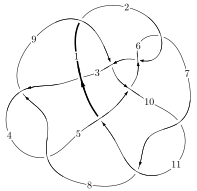
\includegraphics[width=112pt]{../../../GIT/diagram.site/Diagrams/png/577_11a_328.png}\\
\ \ \ A knot diagram\footnotemark}&
\allowdisplaybreaks
\textbf{Linearized knot diagam} \\
\cline{2-2}
 &
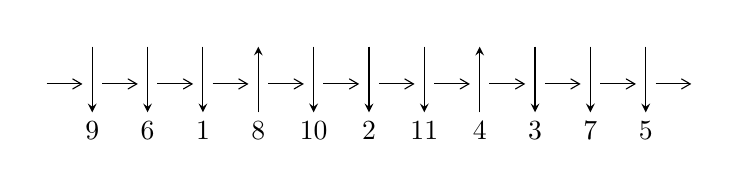
\begin{tikzpicture}[x=20pt, y=17pt]
	% nodes
	\node (C0) at (0, 0) {};
	\node (C1) at (1, 0) {};
	\node (C1U) at (1, +1) {};
	\node (C1D) at (1, -1) {9};

	\node (C2) at (2, 0) {};
	\node (C2U) at (2, +1) {};
	\node (C2D) at (2, -1) {6};

	\node (C3) at (3, 0) {};
	\node (C3U) at (3, +1) {};
	\node (C3D) at (3, -1) {1};

	\node (C4) at (4, 0) {};
	\node (C4U) at (4, +1) {};
	\node (C4D) at (4, -1) {8};

	\node (C5) at (5, 0) {};
	\node (C5U) at (5, +1) {};
	\node (C5D) at (5, -1) {10};

	\node (C6) at (6, 0) {};
	\node (C6U) at (6, +1) {};
	\node (C6D) at (6, -1) {2};

	\node (C7) at (7, 0) {};
	\node (C7U) at (7, +1) {};
	\node (C7D) at (7, -1) {11};

	\node (C8) at (8, 0) {};
	\node (C8U) at (8, +1) {};
	\node (C8D) at (8, -1) {4};

	\node (C9) at (9, 0) {};
	\node (C9U) at (9, +1) {};
	\node (C9D) at (9, -1) {3};

	\node (C10) at (10, 0) {};
	\node (C10U) at (10, +1) {};
	\node (C10D) at (10, -1) {7};

	\node (C11) at (11, 0) {};
	\node (C11U) at (11, +1) {};
	\node (C11D) at (11, -1) {5};
	\node (C12) at (12, 0) {};

	% arrows
	\draw[->,>={angle 60}]
	(C0) edge (C1) (C1) edge (C2) (C2) edge (C3) (C3) edge (C4) (C4) edge (C5) (C5) edge (C6) (C6) edge (C7) (C7) edge (C8) (C8) edge (C9) (C9) edge (C10) (C10) edge (C11) (C11) edge (C12) ;	\draw[->,>=stealth]
	(C1U) edge (C1D) (C2U) edge (C2D) (C3U) edge (C3D) (C4D) edge (C4U) (C5U) edge (C5D) (C6U) edge (C6D) (C7U) edge (C7D) (C8D) edge (C8U) (C9U) edge (C9D) (C10U) edge (C10D) (C11U) edge (C11D) ;
	\end{tikzpicture} \\
\hhline{~~} \\& 
\textbf{Solving Sequence} \\ \cline{2-2} 
 &
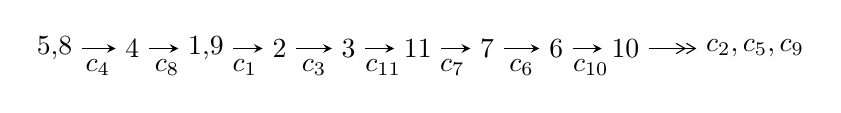
\begin{tikzpicture}[x=25pt, y=7pt]
	% node
	\node (A0) at (-1/8, 0) {5,8};
	\node (A1) at (1, 0) {4};
	\node (A2) at (33/16, 0) {1,9};
	\node (A3) at (25/8, 0) {2};
	\node (A4) at (33/8, 0) {3};
	\node (A5) at (41/8, 0) {11};
	\node (A6) at (49/8, 0) {7};
	\node (A7) at (57/8, 0) {6};
	\node (A8) at (65/8, 0) {10};
	\node (C1) at (1/2, -1) {$c_{4}$};
	\node (C2) at (3/2, -1) {$c_{8}$};
	\node (C3) at (21/8, -1) {$c_{1}$};
	\node (C4) at (29/8, -1) {$c_{3}$};
	\node (C5) at (37/8, -1) {$c_{11}$};
	\node (C6) at (45/8, -1) {$c_{7}$};
	\node (C7) at (53/8, -1) {$c_{6}$};
	\node (C8) at (61/8, -1) {$c_{10}$};
	\node (A9) at (10, 0) {$c_{2},c_{5},c_{9}$};

	% edge
	\draw[->,>=stealth]	
	(A0) edge (A1) (A1) edge (A2) (A2) edge (A3) (A3) edge (A4) (A4) edge (A5) (A5) edge (A6) (A6) edge (A7) (A7) edge (A8) ;
	\draw[->>,>={angle 60}]	
	(A8) edge (A9);
\end{tikzpicture} \\ 

\end{tabular} \\

\footnotetext{
The image of knot diagram is generated by the software ``\textbf{Draw programme}" developed by Andrew Bartholomew(\url{http://www.layer8.co.uk/maths/draw/index.htm\#Running-draw}), where we modified some parts for our purpose(\url{https://github.com/CATsTAILs/LinksPainter}).
}\phantom \\ \newline 
\centering \textbf{Ideals for irreducible components\footnotemark of $X_{\text{par}}$} 
 
\begin{align*}
I^u_{1}&=\langle 
-2.23921\times10^{242} u^{86}-7.92450\times10^{242} u^{85}+\cdots+2.99360\times10^{243} b+1.15001\times10^{243},\\
\phantom{I^u_{1}}&\phantom{= \langle  }2.69979\times10^{242} u^{86}+1.06399\times10^{243} u^{85}+\cdots+5.98721\times10^{243} a-3.98514\times10^{244},\\
\phantom{I^u_{1}}&\phantom{= \langle  }u^{87}+4 u^{86}+\cdots+343 u-49\rangle \\
I^u_{2}&=\langle 
491 u^{12}-351 u^{11}+\cdots+2441 b+3926,\;3175 u^{12}+6674 u^{11}+\cdots+4882 a-4765,\\
\phantom{I^u_{2}}&\phantom{= \langle  }u^{13}+u^{12}+5 u^{11}+5 u^{10}+15 u^9+6 u^8+26 u^7-3 u^6+25 u^5-10 u^4+13 u^3-5 u^2+2 u-1\rangle \\
\\
\end{align*}
\raggedright * 2 irreducible components of $\dim_{\mathbb{C}}=0$, with total 100 representations.\\
\footnotetext{All coefficients of polynomials are rational numbers. But the coefficients are sometimes approximated in decimal forms when there is not enough margin.}
\newpage
\renewcommand{\arraystretch}{1}
\centering \section*{I. $I^u_{1}= \langle -2.24\times10^{242} u^{86}-7.92\times10^{242} u^{85}+\cdots+2.99\times10^{243} b+1.15\times10^{243},\;2.70\times10^{242} u^{86}+1.06\times10^{243} u^{85}+\cdots+5.99\times10^{243} a-3.99\times10^{244},\;u^{87}+4 u^{86}+\cdots+343 u-49 \rangle$}
\flushleft \textbf{(i) Arc colorings}\\
\begin{tabular}{m{7pt} m{180pt} m{7pt} m{180pt} }
\flushright $a_{5}=$&$\begin{pmatrix}1\\0\end{pmatrix}$ \\
\flushright $a_{8}=$&$\begin{pmatrix}0\\u\end{pmatrix}$ \\
\flushright $a_{4}=$&$\begin{pmatrix}1\\u^2\end{pmatrix}$ \\
\flushright $a_{1}=$&$\begin{pmatrix}-0.0450926 u^{86}-0.177711 u^{85}+\cdots-17.8452 u+6.65609\\0.0747999 u^{86}+0.264715 u^{85}+\cdots-0.552281 u-0.384156\end{pmatrix}$ \\
\flushright $a_{9}=$&$\begin{pmatrix}u\\u^3+u\end{pmatrix}$ \\
\flushright $a_{2}=$&$\begin{pmatrix}0.0402372 u^{86}+0.122380 u^{85}+\cdots-33.7223 u+8.81924\\0.0372983 u^{86}+0.116784 u^{85}+\cdots+1.89332 u-0.241227\end{pmatrix}$ \\
\flushright $a_{3}=$&$\begin{pmatrix}-0.0493242 u^{86}-0.246384 u^{85}+\cdots-11.7605 u-0.960720\\0.0348186 u^{86}+0.139522 u^{85}+\cdots-21.6142 u+4.39832\end{pmatrix}$ \\
\flushright $a_{11}=$&$\begin{pmatrix}0.0297073 u^{86}+0.0870039 u^{85}+\cdots-18.3975 u+6.27193\\0.0747999 u^{86}+0.264715 u^{85}+\cdots-0.552281 u-0.384156\end{pmatrix}$ \\
\flushright $a_{7}=$&$\begin{pmatrix}0.0601123 u^{86}+0.192499 u^{85}+\cdots-42.5585 u+12.4589\\-0.0878581 u^{86}-0.355305 u^{85}+\cdots+15.9562 u-1.44904\end{pmatrix}$ \\
\flushright $a_{6}=$&$\begin{pmatrix}0.0993724 u^{86}+0.357805 u^{85}+\cdots-25.6649 u+5.15445\\0.0206546 u^{86}+0.131560 u^{85}+\cdots+0.640094 u+1.53755\end{pmatrix}$ \\
\flushright $a_{10}=$&$\begin{pmatrix}-0.106056 u^{86}-0.436946 u^{85}+\cdots+36.4451 u-8.52379\\-0.0235474 u^{86}-0.0851142 u^{85}+\cdots+9.34856 u-2.37135\end{pmatrix}$\\ \flushright $a_{10}=$&$\begin{pmatrix}-0.106056 u^{86}-0.436946 u^{85}+\cdots+36.4451 u-8.52379\\-0.0235474 u^{86}-0.0851142 u^{85}+\cdots+9.34856 u-2.37135\end{pmatrix}$\\&\end{tabular}
\flushleft \textbf{(ii) Obstruction class $= -1$}\\~\\
\flushleft \textbf{(iii) Cusp Shapes $= 0.108591 u^{86}+0.627995 u^{85}+\cdots-113.643 u+28.5257$}\\~\\
\newpage\renewcommand{\arraystretch}{1}
\flushleft \textbf{(iv) u-Polynomials at the component}\newline \\
\begin{tabular}{m{50pt}|m{274pt}}
Crossings & \hspace{64pt}u-Polynomials at each crossing \\
\hline $$\begin{aligned}c_{1}\end{aligned}$$&$\begin{aligned}
&u^{87}+3 u^{86}+\cdots-5484 u+667
\end{aligned}$\\
\hline $$\begin{aligned}c_{2},c_{6}\end{aligned}$$&$\begin{aligned}
&u^{87}+u^{86}+\cdots-140 u+23
\end{aligned}$\\
\hline $$\begin{aligned}c_{3}\end{aligned}$$&$\begin{aligned}
&2(2 u^{87}-17 u^{86}+\cdots-8 u+1)
\end{aligned}$\\
\hline $$\begin{aligned}c_{4},c_{8}\end{aligned}$$&$\begin{aligned}
&u^{87}-4 u^{86}+\cdots+343 u+49
\end{aligned}$\\
\hline $$\begin{aligned}c_{5}\end{aligned}$$&$\begin{aligned}
&u^{87}-3 u^{86}+\cdots+11633 u+2362
\end{aligned}$\\
\hline $$\begin{aligned}c_{7},c_{10}\end{aligned}$$&$\begin{aligned}
&2(2 u^{87}+5 u^{86}+\cdots+9624 u+539)
\end{aligned}$\\
\hline $$\begin{aligned}c_{9}\end{aligned}$$&$\begin{aligned}
&2(2 u^{87}-5 u^{86}+\cdots+1311 u+349)
\end{aligned}$\\
\hline $$\begin{aligned}c_{11}\end{aligned}$$&$\begin{aligned}
&u^{87}+2 u^{86}+\cdots+2885 u+538
\end{aligned}$\\
\hline
\end{tabular}\\~\\
\newpage\renewcommand{\arraystretch}{1}
\flushleft \textbf{(v) Riley Polynomials at the component}\newline \\
\begin{tabular}{m{50pt}|m{274pt}}
Crossings & \hspace{64pt}Riley Polynomials at each crossing \\
\hline $$\begin{aligned}c_{1}\end{aligned}$$&$\begin{aligned}
&y^{87}-13 y^{86}+\cdots+17748096 y-444889
\end{aligned}$\\
\hline $$\begin{aligned}c_{2},c_{6}\end{aligned}$$&$\begin{aligned}
&y^{87}+45 y^{86}+\cdots+11504 y-529
\end{aligned}$\\
\hline $$\begin{aligned}c_{3}\end{aligned}$$&$\begin{aligned}
&4(4 y^{87}-13 y^{86}+\cdots-4 y-1)
\end{aligned}$\\
\hline $$\begin{aligned}c_{4},c_{8}\end{aligned}$$&$\begin{aligned}
&y^{87}+66 y^{86}+\cdots+43561 y-2401
\end{aligned}$\\
\hline $$\begin{aligned}c_{5}\end{aligned}$$&$\begin{aligned}
&y^{87}+9 y^{86}+\cdots-55400087 y-5579044
\end{aligned}$\\
\hline $$\begin{aligned}c_{7},c_{10}\end{aligned}$$&$\begin{aligned}
&4(4 y^{87}-285 y^{86}+\cdots+1.28127\times10^{7} y-290521)
\end{aligned}$\\
\hline $$\begin{aligned}c_{9}\end{aligned}$$&$\begin{aligned}
&4(4 y^{87}+103 y^{86}+\cdots-1.77548\times10^{7} y-121801)
\end{aligned}$\\
\hline $$\begin{aligned}c_{11}\end{aligned}$$&$\begin{aligned}
&y^{87}-38 y^{86}+\cdots+7135321 y-289444
\end{aligned}$\\
\hline
\end{tabular}\\~\\
\newpage\flushleft \textbf{(vi) Complex Volumes and Cusp Shapes}
$$\begin{array}{c|c|c}  
\text{Solutions to }I^u_{1}& \I (\text{vol} + \sqrt{-1}CS) & \text{Cusp shape}\\
 \hline 
\begin{aligned}
u &= -0.776879 + 0.541054 I \\
a &= \phantom{-}0.188536 + 1.157520 I \\
b &= \phantom{-}1.026510 - 0.627724 I\end{aligned}
 & \phantom{-}1.01962 + 3.49300 I & \phantom{-0.000000 } 0 \\ \hline\begin{aligned}
u &= -0.776879 - 0.541054 I \\
a &= \phantom{-}0.188536 - 1.157520 I \\
b &= \phantom{-}1.026510 + 0.627724 I\end{aligned}
 & \phantom{-}1.01962 - 3.49300 I & \phantom{-0.000000 } 0 \\ \hline\begin{aligned}
u &= \phantom{-}1.007580 + 0.327641 I \\
a &= \phantom{-}0.183992 + 0.069606 I \\
b &= \phantom{-}0.789772 - 0.734118 I\end{aligned}
 & -1.60864 + 6.07731 I & \phantom{-0.000000 } 0 \\ \hline\begin{aligned}
u &= \phantom{-}1.007580 - 0.327641 I \\
a &= \phantom{-}0.183992 - 0.069606 I \\
b &= \phantom{-}0.789772 + 0.734118 I\end{aligned}
 & -1.60864 - 6.07731 I & \phantom{-0.000000 } 0 \\ \hline\begin{aligned}
u &= \phantom{-}0.245817 + 0.897592 I \\
a &= \phantom{-}1.80503 - 0.59455 I \\
b &= -0.938277 + 0.817700 I\end{aligned}
 & \phantom{-}3.46748 + 3.58811 I & \phantom{-0.000000 } 0 \\ \hline\begin{aligned}
u &= \phantom{-}0.245817 - 0.897592 I \\
a &= \phantom{-}1.80503 + 0.59455 I \\
b &= -0.938277 - 0.817700 I\end{aligned}
 & \phantom{-}3.46748 - 3.58811 I & \phantom{-0.000000 } 0 \\ \hline\begin{aligned}
u &= \phantom{-}0.908219 + 0.099499 I \\
a &= \phantom{-}0.364543 - 0.135798 I \\
b &= -0.390262 - 0.953575 I\end{aligned}
 & \phantom{-}5.02660 - 6.57361 I & \phantom{-0.000000 } 0 \\ \hline\begin{aligned}
u &= \phantom{-}0.908219 - 0.099499 I \\
a &= \phantom{-}0.364543 + 0.135798 I \\
b &= -0.390262 + 0.953575 I\end{aligned}
 & \phantom{-}5.02660 + 6.57361 I & \phantom{-0.000000 } 0 \\ \hline\begin{aligned}
u &= -0.374562 + 1.029910 I \\
a &= \phantom{-}1.97132 - 0.41269 I \\
b &= -2.04798 - 0.80570 I\end{aligned}
 & -0.50770 - 7.93768 I & \phantom{-0.000000 } 0 \\ \hline\begin{aligned}
u &= -0.374562 - 1.029910 I \\
a &= \phantom{-}1.97132 + 0.41269 I \\
b &= -2.04798 + 0.80570 I\end{aligned}
 & -0.50770 + 7.93768 I & \phantom{-0.000000 } 0\\
 \hline 
 \end{array}$$\newpage$$\begin{array}{c|c|c}  
\text{Solutions to }I^u_{1}& \I (\text{vol} + \sqrt{-1}CS) & \text{Cusp shape}\\
 \hline 
\begin{aligned}
u &= -0.217099 + 1.081390 I \\
a &= -1.90936 + 0.88490 I \\
b &= \phantom{-}0.529903 + 0.247555 I\end{aligned}
 & -0.703925 - 0.037215 I & \phantom{-0.000000 } 0 \\ \hline\begin{aligned}
u &= -0.217099 - 1.081390 I \\
a &= -1.90936 - 0.88490 I \\
b &= \phantom{-}0.529903 - 0.247555 I\end{aligned}
 & -0.703925 + 0.037215 I & \phantom{-0.000000 } 0 \\ \hline\begin{aligned}
u &= -0.220013 + 1.097370 I \\
a &= -0.953091 - 0.049330 I \\
b &= \phantom{-}0.613788 + 0.509488 I\end{aligned}
 & -0.94053 - 1.58665 I & \phantom{-0.000000 } 0 \\ \hline\begin{aligned}
u &= -0.220013 - 1.097370 I \\
a &= -0.953091 + 0.049330 I \\
b &= \phantom{-}0.613788 - 0.509488 I\end{aligned}
 & -0.94053 + 1.58665 I & \phantom{-0.000000 } 0 \\ \hline\begin{aligned}
u &= -0.027487 + 1.147150 I \\
a &= -0.068691 - 0.603804 I \\
b &= \phantom{-}0.109168 - 1.084490 I\end{aligned}
 & -2.95518 - 0.92414 I & \phantom{-0.000000 } 0 \\ \hline\begin{aligned}
u &= -0.027487 - 1.147150 I \\
a &= -0.068691 + 0.603804 I \\
b &= \phantom{-}0.109168 + 1.084490 I\end{aligned}
 & -2.95518 + 0.92414 I & \phantom{-0.000000 } 0 \\ \hline\begin{aligned}
u &= -0.834059 + 0.034209 I \\
a &= -0.225565 - 0.290060 I \\
b &= -0.822239 + 0.737364 I\end{aligned}
 & \phantom{-}3.93560 + 2.19338 I & -1.92699 - 3.84180 I \\ \hline\begin{aligned}
u &= -0.834059 - 0.034209 I \\
a &= -0.225565 + 0.290060 I \\
b &= -0.822239 - 0.737364 I\end{aligned}
 & \phantom{-}3.93560 - 2.19338 I & -1.92699 + 3.84180 I \\ \hline\begin{aligned}
u &= \phantom{-}0.202235 + 1.161160 I \\
a &= -1.79634 + 0.72293 I \\
b &= \phantom{-}0.802586 - 0.468686 I\end{aligned}
 & \phantom{-}2.03222 + 0.78901 I & \phantom{-0.000000 } 0 \\ \hline\begin{aligned}
u &= \phantom{-}0.202235 - 1.161160 I \\
a &= -1.79634 - 0.72293 I \\
b &= \phantom{-}0.802586 + 0.468686 I\end{aligned}
 & \phantom{-}2.03222 - 0.78901 I & \phantom{-0.000000 } 0\\
 \hline 
 \end{array}$$\newpage$$\begin{array}{c|c|c}  
\text{Solutions to }I^u_{1}& \I (\text{vol} + \sqrt{-1}CS) & \text{Cusp shape}\\
 \hline 
\begin{aligned}
u &= \phantom{-}0.012862 + 1.192010 I \\
a &= -1.90807 - 0.84701 I \\
b &= \phantom{-}1.94746 + 1.83329 I\end{aligned}
 & -3.17906 + 6.66017 I & \phantom{-0.000000 } 0 \\ \hline\begin{aligned}
u &= \phantom{-}0.012862 - 1.192010 I \\
a &= -1.90807 + 0.84701 I \\
b &= \phantom{-}1.94746 - 1.83329 I\end{aligned}
 & -3.17906 - 6.66017 I & \phantom{-0.000000 } 0 \\ \hline\begin{aligned}
u &= \phantom{-}0.235984 + 1.200170 I \\
a &= \phantom{-}1.48127 + 0.13165 I \\
b &= -0.951440 - 0.148069 I\end{aligned}
 & -4.06130 + 2.44977 I & \phantom{-0.000000 } 0 \\ \hline\begin{aligned}
u &= \phantom{-}0.235984 - 1.200170 I \\
a &= \phantom{-}1.48127 - 0.13165 I \\
b &= -0.951440 + 0.148069 I\end{aligned}
 & -4.06130 - 2.44977 I & \phantom{-0.000000 } 0 \\ \hline\begin{aligned}
u &= \phantom{-}0.761682 + 0.143291 I \\
a &= -0.976859 + 0.023521 I \\
b &= -0.563074 + 0.406965 I\end{aligned}
 & -1.92081 + 0.61884 I & -7.87734 - 1.96780 I \\ \hline\begin{aligned}
u &= \phantom{-}0.761682 - 0.143291 I \\
a &= -0.976859 - 0.023521 I \\
b &= -0.563074 - 0.406965 I\end{aligned}
 & -1.92081 - 0.61884 I & -7.87734 + 1.96780 I \\ \hline\begin{aligned}
u &= \phantom{-}0.112847 + 1.223690 I \\
a &= \phantom{-}2.47523 - 0.15334 I \\
b &= -2.44222 + 1.06035 I\end{aligned}
 & -7.01048 + 0.84605 I & \phantom{-0.000000 } 0 \\ \hline\begin{aligned}
u &= \phantom{-}0.112847 - 1.223690 I \\
a &= \phantom{-}2.47523 + 0.15334 I \\
b &= -2.44222 - 1.06035 I\end{aligned}
 & -7.01048 - 0.84605 I & \phantom{-0.000000 } 0 \\ \hline\begin{aligned}
u &= -0.755476 + 0.104993 I \\
a &= -0.419450 - 0.027979 I \\
b &= \phantom{-}0.223634 + 0.914975 I\end{aligned}
 & \phantom{-}1.83703 - 2.21620 I & -3.51529 + 3.55324 I \\ \hline\begin{aligned}
u &= -0.755476 - 0.104993 I \\
a &= -0.419450 + 0.027979 I \\
b &= \phantom{-}0.223634 - 0.914975 I\end{aligned}
 & \phantom{-}1.83703 + 2.21620 I & -3.51529 - 3.55324 I\\
 \hline 
 \end{array}$$\newpage$$\begin{array}{c|c|c}  
\text{Solutions to }I^u_{1}& \I (\text{vol} + \sqrt{-1}CS) & \text{Cusp shape}\\
 \hline 
\begin{aligned}
u &= -1.210730 + 0.265007 I \\
a &= -0.113980 + 0.093687 I \\
b &= -0.811339 - 0.684971 I\end{aligned}
 & \phantom{-}1.28183 - 11.73510 I & \phantom{-0.000000 } 0 \\ \hline\begin{aligned}
u &= -1.210730 - 0.265007 I \\
a &= -0.113980 - 0.093687 I \\
b &= -0.811339 + 0.684971 I\end{aligned}
 & \phantom{-}1.28183 + 11.73510 I & \phantom{-0.000000 } 0 \\ \hline\begin{aligned}
u &= -0.370860 + 1.187910 I \\
a &= -1.44787 + 0.53047 I \\
b &= \phantom{-}1.49725 - 0.21594 I\end{aligned}
 & -0.72894 - 6.29842 I & \phantom{-0.000000 } 0 \\ \hline\begin{aligned}
u &= -0.370860 - 1.187910 I \\
a &= -1.44787 - 0.53047 I \\
b &= \phantom{-}1.49725 + 0.21594 I\end{aligned}
 & -0.72894 + 6.29842 I & \phantom{-0.000000 } 0 \\ \hline\begin{aligned}
u &= \phantom{-}0.082178 + 1.267230 I \\
a &= \phantom{-}1.81882 + 0.60579 I \\
b &= -1.43238 + 0.41505 I\end{aligned}
 & -7.65344 + 1.93513 I & \phantom{-0.000000 } 0 \\ \hline\begin{aligned}
u &= \phantom{-}0.082178 - 1.267230 I \\
a &= \phantom{-}1.81882 - 0.60579 I \\
b &= -1.43238 - 0.41505 I\end{aligned}
 & -7.65344 - 1.93513 I & \phantom{-0.000000 } 0 \\ \hline\begin{aligned}
u &= \phantom{-}0.154767 + 1.267260 I \\
a &= -1.123800 + 0.806234 I \\
b &= \phantom{-}1.16362 - 1.85704 I\end{aligned}
 & -6.42084 + 3.25398 I & \phantom{-0.000000 } 0 \\ \hline\begin{aligned}
u &= \phantom{-}0.154767 - 1.267260 I \\
a &= -1.123800 - 0.806234 I \\
b &= \phantom{-}1.16362 + 1.85704 I\end{aligned}
 & -6.42084 - 3.25398 I & \phantom{-0.000000 } 0 \\ \hline\begin{aligned}
u &= \phantom{-}0.315271 + 0.626744 I \\
a &= \phantom{-}0.014758 - 0.894661 I \\
b &= \phantom{-}0.34862 + 1.39642 I\end{aligned}
 & \phantom{-}4.42600 - 0.87222 I & -1.33257 - 4.60840 I \\ \hline\begin{aligned}
u &= \phantom{-}0.315271 - 0.626744 I \\
a &= \phantom{-}0.014758 + 0.894661 I \\
b &= \phantom{-}0.34862 - 1.39642 I\end{aligned}
 & \phantom{-}4.42600 + 0.87222 I & -1.33257 + 4.60840 I\\
 \hline 
 \end{array}$$\newpage$$\begin{array}{c|c|c}  
\text{Solutions to }I^u_{1}& \I (\text{vol} + \sqrt{-1}CS) & \text{Cusp shape}\\
 \hline 
\begin{aligned}
u &= -0.138100 + 1.293420 I \\
a &= -1.55432 + 0.54367 I \\
b &= \phantom{-}1.168620 + 0.682207 I\end{aligned}
 & -4.91824 - 8.48201 I & \phantom{-0.000000 } 0 \\ \hline\begin{aligned}
u &= -0.138100 - 1.293420 I \\
a &= -1.55432 - 0.54367 I \\
b &= \phantom{-}1.168620 - 0.682207 I\end{aligned}
 & -4.91824 + 8.48201 I & \phantom{-0.000000 } 0 \\ \hline\begin{aligned}
u &= \phantom{-}0.428306 + 1.245240 I \\
a &= -1.62246 + 0.15416 I \\
b &= \phantom{-}0.755026 - 0.694879 I\end{aligned}
 & \phantom{-}1.44453 + 11.33890 I & \phantom{-0.000000 } 0 \\ \hline\begin{aligned}
u &= \phantom{-}0.428306 - 1.245240 I \\
a &= -1.62246 - 0.15416 I \\
b &= \phantom{-}0.755026 + 0.694879 I\end{aligned}
 & \phantom{-}1.44453 - 11.33890 I & \phantom{-0.000000 } 0 \\ \hline\begin{aligned}
u &= \phantom{-}0.181300 + 1.304480 I \\
a &= -0.363009 - 0.100801 I \\
b &= \phantom{-}0.459339 - 0.988301 I\end{aligned}
 & -6.35047 + 2.80896 I & \phantom{-0.000000 } 0 \\ \hline\begin{aligned}
u &= \phantom{-}0.181300 - 1.304480 I \\
a &= -0.363009 + 0.100801 I \\
b &= \phantom{-}0.459339 + 0.988301 I\end{aligned}
 & -6.35047 - 2.80896 I & \phantom{-0.000000 } 0 \\ \hline\begin{aligned}
u &= -0.388024 + 1.265100 I \\
a &= -1.80417 + 0.04080 I \\
b &= \phantom{-}1.63904 + 0.82465 I\end{aligned}
 & \phantom{-}0.10297 - 6.59252 I & \phantom{-0.000000 } 0 \\ \hline\begin{aligned}
u &= -0.388024 - 1.265100 I \\
a &= -1.80417 - 0.04080 I \\
b &= \phantom{-}1.63904 - 0.82465 I\end{aligned}
 & \phantom{-}0.10297 + 6.59252 I & \phantom{-0.000000 } 0 \\ \hline\begin{aligned}
u &= -0.328530 + 1.294480 I \\
a &= \phantom{-}1.49353 + 0.38820 I \\
b &= -0.815892 - 0.631455 I\end{aligned}
 & -2.48697 - 6.11850 I & \phantom{-0.000000 } 0 \\ \hline\begin{aligned}
u &= -0.328530 - 1.294480 I \\
a &= \phantom{-}1.49353 - 0.38820 I \\
b &= -0.815892 + 0.631455 I\end{aligned}
 & -2.48697 + 6.11850 I & \phantom{-0.000000 } 0\\
 \hline 
 \end{array}$$\newpage$$\begin{array}{c|c|c}  
\text{Solutions to }I^u_{1}& \I (\text{vol} + \sqrt{-1}CS) & \text{Cusp shape}\\
 \hline 
\begin{aligned}
u &= \phantom{-}0.012517 + 1.341530 I \\
a &= \phantom{-}0.877313 - 0.120821 I \\
b &= -0.758450 - 0.797102 I\end{aligned}
 & -6.25662 + 2.11272 I & \phantom{-0.000000 } 0 \\ \hline\begin{aligned}
u &= \phantom{-}0.012517 - 1.341530 I \\
a &= \phantom{-}0.877313 + 0.120821 I \\
b &= -0.758450 + 0.797102 I\end{aligned}
 & -6.25662 - 2.11272 I & \phantom{-0.000000 } 0 \\ \hline\begin{aligned}
u &= \phantom{-}1.354960 + 0.065636 I \\
a &= -0.249415 - 0.140378 I \\
b &= -0.659999 + 0.151798 I\end{aligned}
 & -2.16816 + 0.86837 I & \phantom{-0.000000 } 0 \\ \hline\begin{aligned}
u &= \phantom{-}1.354960 - 0.065636 I \\
a &= -0.249415 + 0.140378 I \\
b &= -0.659999 - 0.151798 I\end{aligned}
 & -2.16816 - 0.86837 I & \phantom{-0.000000 } 0 \\ \hline\begin{aligned}
u &= \phantom{-}0.100175 + 0.612166 I \\
a &= \phantom{-}0.37206 + 2.60657 I \\
b &= -0.273208 + 0.157111 I\end{aligned}
 & -1.084890 + 0.871384 I & -15.6106 - 3.4978 I \\ \hline\begin{aligned}
u &= \phantom{-}0.100175 - 0.612166 I \\
a &= \phantom{-}0.37206 - 2.60657 I \\
b &= -0.273208 - 0.157111 I\end{aligned}
 & -1.084890 - 0.871384 I & -15.6106 + 3.4978 I \\ \hline\begin{aligned}
u &= -0.67656 + 1.24255 I \\
a &= \phantom{-}0.0242517 - 0.0831628 I \\
b &= \phantom{-}0.012280 + 0.372469 I\end{aligned}
 & -0.78893 - 2.23324 I & \phantom{-0.000000 } 0 \\ \hline\begin{aligned}
u &= -0.67656 - 1.24255 I \\
a &= \phantom{-}0.0242517 + 0.0831628 I \\
b &= \phantom{-}0.012280 - 0.372469 I\end{aligned}
 & -0.78893 + 2.23324 I & \phantom{-0.000000 } 0 \\ \hline\begin{aligned}
u &= -0.543318 + 0.090886 I \\
a &= \phantom{-}0.411855 - 1.155200 I \\
b &= -0.757344 - 0.051881 I\end{aligned}
 & \phantom{-}2.36842 + 2.62824 I & -3.63497 - 2.44788 I \\ \hline\begin{aligned}
u &= -0.543318 - 0.090886 I \\
a &= \phantom{-}0.411855 + 1.155200 I \\
b &= -0.757344 + 0.051881 I\end{aligned}
 & \phantom{-}2.36842 - 2.62824 I & -3.63497 + 2.44788 I\\
 \hline 
 \end{array}$$\newpage$$\begin{array}{c|c|c}  
\text{Solutions to }I^u_{1}& \I (\text{vol} + \sqrt{-1}CS) & \text{Cusp shape}\\
 \hline 
\begin{aligned}
u &= \phantom{-}0.42905 + 1.44683 I \\
a &= \phantom{-}1.54404 - 0.21136 I \\
b &= -1.51558 + 1.17301 I\end{aligned}
 & -7.14017 + 11.20710 I & \phantom{-0.000000 } 0 \\ \hline\begin{aligned}
u &= \phantom{-}0.42905 - 1.44683 I \\
a &= \phantom{-}1.54404 + 0.21136 I \\
b &= -1.51558 - 1.17301 I\end{aligned}
 & -7.14017 - 11.20710 I & \phantom{-0.000000 } 0 \\ \hline\begin{aligned}
u &= \phantom{-}0.43735 + 1.45185 I \\
a &= -1.149860 - 0.022344 I \\
b &= \phantom{-}1.21403 - 0.98521 I\end{aligned}
 & -7.95756 + 5.21172 I & \phantom{-0.000000 } 0 \\ \hline\begin{aligned}
u &= \phantom{-}0.43735 - 1.45185 I \\
a &= -1.149860 + 0.022344 I \\
b &= \phantom{-}1.21403 + 0.98521 I\end{aligned}
 & -7.95756 - 5.21172 I & \phantom{-0.000000 } 0 \\ \hline\begin{aligned}
u &= -0.12280 + 1.51626 I \\
a &= -0.377043 + 0.062903 I \\
b &= \phantom{-}0.441833 + 0.292673 I\end{aligned}
 & -0.68412 - 1.98002 I & \phantom{-0.000000 } 0 \\ \hline\begin{aligned}
u &= -0.12280 - 1.51626 I \\
a &= -0.377043 - 0.062903 I \\
b &= \phantom{-}0.441833 - 0.292673 I\end{aligned}
 & -0.68412 + 1.98002 I & \phantom{-0.000000 } 0 \\ \hline\begin{aligned}
u &= \phantom{-}0.403739 + 0.208025 I \\
a &= \phantom{-}0.804446 - 0.453238 I \\
b &= -0.259208 - 1.215850 I\end{aligned}
 & \phantom{-}4.93158 + 1.73284 I & \phantom{-}1.22516 - 5.83487 I \\ \hline\begin{aligned}
u &= \phantom{-}0.403739 - 0.208025 I \\
a &= \phantom{-}0.804446 + 0.453238 I \\
b &= -0.259208 + 1.215850 I\end{aligned}
 & \phantom{-}4.93158 - 1.73284 I & \phantom{-}1.22516 + 5.83487 I \\ \hline\begin{aligned}
u &= -0.50070 + 1.46622 I \\
a &= -1.44297 - 0.11937 I \\
b &= \phantom{-}1.43093 + 1.14290 I\end{aligned}
 & -4.1159 - 17.6919 I & \phantom{-0.000000 } 0 \\ \hline\begin{aligned}
u &= -0.50070 - 1.46622 I \\
a &= -1.44297 + 0.11937 I \\
b &= \phantom{-}1.43093 - 1.14290 I\end{aligned}
 & -4.1159 + 17.6919 I & \phantom{-0.000000 } 0\\
 \hline 
 \end{array}$$\newpage$$\begin{array}{c|c|c}  
\text{Solutions to }I^u_{1}& \I (\text{vol} + \sqrt{-1}CS) & \text{Cusp shape}\\
 \hline 
\begin{aligned}
u &= \phantom{-}0.60050 + 1.43503 I \\
a &= -1.090220 - 0.150328 I \\
b &= \phantom{-}1.36060 - 0.72302 I\end{aligned}
 & -6.65882 + 7.54335 I & \phantom{-0.000000 } 0 \\ \hline\begin{aligned}
u &= \phantom{-}0.60050 - 1.43503 I \\
a &= -1.090220 + 0.150328 I \\
b &= \phantom{-}1.36060 + 0.72302 I\end{aligned}
 & -6.65882 - 7.54335 I & \phantom{-0.000000 } 0 \\ \hline\begin{aligned}
u &= -0.49169 + 1.48005 I \\
a &= \phantom{-}1.152940 - 0.055999 I \\
b &= -1.09293 - 0.91892 I\end{aligned}
 & -6.98154 - 8.93541 I & \phantom{-0.000000 } 0 \\ \hline\begin{aligned}
u &= -0.49169 - 1.48005 I \\
a &= \phantom{-}1.152940 + 0.055999 I \\
b &= -1.09293 + 0.91892 I\end{aligned}
 & -6.98154 + 8.93541 I & \phantom{-0.000000 } 0 \\ \hline\begin{aligned}
u &= \phantom{-}0.283569 + 0.325822 I \\
a &= -0.86667 + 2.61101 I \\
b &= \phantom{-}0.219477 + 0.269391 I\end{aligned}
 & -1.04332 + 1.10567 I & -9.46807 + 3.92768 I \\ \hline\begin{aligned}
u &= \phantom{-}0.283569 - 0.325822 I \\
a &= -0.86667 - 2.61101 I \\
b &= \phantom{-}0.219477 - 0.269391 I\end{aligned}
 & -1.04332 - 1.10567 I & -9.46807 - 3.92768 I \\ \hline\begin{aligned}
u &= -0.52905 + 1.51463 I \\
a &= \phantom{-}1.050270 - 0.039593 I \\
b &= -1.218100 - 0.659542 I\end{aligned}
 & -6.59608 - 4.70222 I & \phantom{-0.000000 } 0 \\ \hline\begin{aligned}
u &= -0.52905 - 1.51463 I \\
a &= \phantom{-}1.050270 + 0.039593 I \\
b &= -1.218100 + 0.659542 I\end{aligned}
 & -6.59608 + 4.70222 I & \phantom{-0.000000 } 0 \\ \hline\begin{aligned}
u &= \phantom{-}0.354922\phantom{ +0.000000I} \\
a &= -1.12692\phantom{ +0.000000I} \\
b &= \phantom{-}0.380191\phantom{ +0.000000I}\end{aligned}
 & -0.829400\phantom{ +0.000000I} & -12.4500\phantom{ +0.000000I} \\ \hline\begin{aligned}
u &= \phantom{-}0.294507 + 0.068923 I \\
a &= \phantom{-}1.91812 - 1.72593 I \\
b &= \phantom{-}1.327900 + 0.309964 I\end{aligned}
 & -3.55911 + 0.66256 I & -6.82987 - 9.28934 I\\
 \hline 
 \end{array}$$\newpage$$\begin{array}{c|c|c}  
\text{Solutions to }I^u_{1}& \I (\text{vol} + \sqrt{-1}CS) & \text{Cusp shape}\\
 \hline 
\begin{aligned}
u &= \phantom{-}0.294507 - 0.068923 I \\
a &= \phantom{-}1.91812 + 1.72593 I \\
b &= \phantom{-}1.327900 - 0.309964 I\end{aligned}
 & -3.55911 - 0.66256 I & -6.82987 + 9.28934 I \\ \hline\begin{aligned}
u &= -0.206735 + 0.210541 I \\
a &= -0.51301 - 4.12782 I \\
b &= -1.264930 + 0.200555 I\end{aligned}
 & -0.32476 - 6.96628 I & -7.63597 + 5.26059 I \\ \hline\begin{aligned}
u &= -0.206735 - 0.210541 I \\
a &= -0.51301 + 4.12782 I \\
b &= -1.264930 - 0.200555 I\end{aligned}
 & -0.32476 + 6.96628 I & -7.63597 - 5.26059 I \\ \hline\begin{aligned}
u &= -1.88839 + 0.16543 I \\
a &= \phantom{-}0.0280191 + 0.0598057 I \\
b &= \phantom{-}0.473251 + 0.100354 I\end{aligned}
 & -1.16868 - 2.46445 I & \phantom{-0.000000 } 0 \\ \hline\begin{aligned}
u &= -1.88839 - 0.16543 I \\
a &= \phantom{-}0.0280191 - 0.0598057 I \\
b &= \phantom{-}0.473251 - 0.100354 I\end{aligned}
 & -1.16868 + 2.46445 I & \phantom{-0.000000 } 0 \\ \hline\begin{aligned}
u &= -0.14180 + 1.98107 I \\
a &= -0.190656 - 0.343084 I \\
b &= \phantom{-}0.270083 + 0.903599 I\end{aligned}
 & -2.44085 + 2.75616 I & \phantom{-0.000000 } 0 \\ \hline\begin{aligned}
u &= -0.14180 - 1.98107 I \\
a &= -0.190656 + 0.343084 I \\
b &= \phantom{-}0.270083 - 0.903599 I\end{aligned}
 & -2.44085 - 2.75616 I & \phantom{-0.000000 } 0\\
 \hline 
 \end{array}$$\newpage\newpage\renewcommand{\arraystretch}{1}
\centering \section*{II. $I^u_{2}= \langle 491 u^{12}-351 u^{11}+\cdots+2441 b+3926,\;3175 u^{12}+6674 u^{11}+\cdots+4882 a-4765,\;u^{13}+u^{12}+\cdots+2 u-1 \rangle$}
\flushleft \textbf{(i) Arc colorings}\\
\begin{tabular}{m{7pt} m{180pt} m{7pt} m{180pt} }
\flushright $a_{5}=$&$\begin{pmatrix}1\\0\end{pmatrix}$ \\
\flushright $a_{8}=$&$\begin{pmatrix}0\\u\end{pmatrix}$ \\
\flushright $a_{4}=$&$\begin{pmatrix}1\\u^2\end{pmatrix}$ \\
\flushright $a_{1}=$&$\begin{pmatrix}-0.650348 u^{12}-1.36706 u^{11}+\cdots-1.98382 u+0.976034\\-0.201147 u^{12}+0.143794 u^{11}+\cdots+3.64154 u-1.60836\end{pmatrix}$ \\
\flushright $a_{9}=$&$\begin{pmatrix}u\\u^3+u\end{pmatrix}$ \\
\flushright $a_{2}=$&$\begin{pmatrix}-0.495494 u^{12}-0.779189 u^{11}+\cdots-0.591766 u+0.104261\\-0.261368 u^{12}+0.192954 u^{11}+\cdots+4.32241 u-2.04711\end{pmatrix}$ \\
\flushright $a_{3}=$&$\begin{pmatrix}0.880479 u^{12}+1.39349 u^{11}+\cdots-3.72522 u+0.700635\\-0.612864 u^{12}-1.03032 u^{11}+\cdots-0.519869 u+0.820565\end{pmatrix}$ \\
\flushright $a_{11}=$&$\begin{pmatrix}-0.851495 u^{12}-1.22327 u^{11}+\cdots+1.65772 u-0.632323\\-0.201147 u^{12}+0.143794 u^{11}+\cdots+3.64154 u-1.60836\end{pmatrix}$ \\
\flushright $a_{7}=$&$\begin{pmatrix}0.744879 u^{12}+1.74908 u^{11}+\cdots+1.39973 u-0.573023\\0.798853 u^{12}+1.14379 u^{11}+\cdots-0.358460 u+0.391643\end{pmatrix}$ \\
\flushright $a_{6}=$&$\begin{pmatrix}0.0437321 u^{12}+0.892872 u^{11}+\cdots+3.54127 u-1.68138\\1.35190 u^{12}+1.24334 u^{11}+\cdots-4.52970 u+0.278165\end{pmatrix}$ \\
\flushright $a_{10}=$&$\begin{pmatrix}-0.978748 u^{12}-0.0836747 u^{11}+\cdots+5.32861 u-2.05945\\0.196641 u^{12}+0.635395 u^{11}+\cdots+3.45023 u-0.995903\end{pmatrix}$\\ \flushright $a_{10}=$&$\begin{pmatrix}-0.978748 u^{12}-0.0836747 u^{11}+\cdots+5.32861 u-2.05945\\0.196641 u^{12}+0.635395 u^{11}+\cdots+3.45023 u-0.995903\end{pmatrix}$\\&\end{tabular}
\flushleft \textbf{(ii) Obstruction class $= 1$}\\~\\
\flushleft \textbf{(iii) Cusp Shapes $= -\frac{33641}{39056} u^{12}-\frac{24777}{19528} u^{11}+\cdots-\frac{452231}{39056} u-\frac{213017}{39056}$}\\~\\
\newpage\renewcommand{\arraystretch}{1}
\flushleft \textbf{(iv) u-Polynomials at the component}\newline \\
\begin{tabular}{m{50pt}|m{274pt}}
Crossings & \hspace{64pt}u-Polynomials at each crossing \\
\hline $$\begin{aligned}c_{1}\end{aligned}$$&$\begin{aligned}
&u^{13}-2 u^{12}+\cdots+7 u+1
\end{aligned}$\\
\hline $$\begin{aligned}c_{2}\end{aligned}$$&$\begin{aligned}
&u^{13}+2 u^{12}+\cdots+u-1
\end{aligned}$\\
\hline $$\begin{aligned}c_{3}\end{aligned}$$&$\begin{aligned}
&2(2 u^{13}+5 u^{12}+\cdots+7 u+1)
\end{aligned}$\\
\hline $$\begin{aligned}c_{4}\end{aligned}$$&$\begin{aligned}
&u^{13}+u^{12}+\cdots+2 u-1
\end{aligned}$\\
\hline $$\begin{aligned}c_{5}\end{aligned}$$&$\begin{aligned}
&u^{13}+2 u^{12}+\cdots- u-2
\end{aligned}$\\
\hline $$\begin{aligned}c_{6}\end{aligned}$$&$\begin{aligned}
&u^{13}-2 u^{12}+\cdots+u+1
\end{aligned}$\\
\hline $$\begin{aligned}c_{7}\end{aligned}$$&$\begin{aligned}
&2(2 u^{13}+u^{12}+\cdots+13 u-5)
\end{aligned}$\\
\hline $$\begin{aligned}c_{8}\end{aligned}$$&$\begin{aligned}
&u^{13}- u^{12}+\cdots+2 u+1
\end{aligned}$\\
\hline $$\begin{aligned}c_{9}\end{aligned}$$&$\begin{aligned}
&2(2 u^{13}- u^{12}+\cdots+6 u+1)
\end{aligned}$\\
\hline $$\begin{aligned}c_{10}\end{aligned}$$&$\begin{aligned}
&2(2 u^{13}- u^{12}+\cdots+13 u+5)
\end{aligned}$\\
\hline $$\begin{aligned}c_{11}\end{aligned}$$&$\begin{aligned}
&u^{13}+u^{12}+\cdots-5 u-2
\end{aligned}$\\
\hline
\end{tabular}\\~\\
\newpage\renewcommand{\arraystretch}{1}
\flushleft \textbf{(v) Riley Polynomials at the component}\newline \\
\begin{tabular}{m{50pt}|m{274pt}}
Crossings & \hspace{64pt}Riley Polynomials at each crossing \\
\hline $$\begin{aligned}c_{1}\end{aligned}$$&$\begin{aligned}
&y^{13}+2 y^{12}+\cdots+25 y-1
\end{aligned}$\\
\hline $$\begin{aligned}c_{2},c_{6}\end{aligned}$$&$\begin{aligned}
&y^{13}+4 y^{12}+\cdots-11 y-1
\end{aligned}$\\
\hline $$\begin{aligned}c_{3}\end{aligned}$$&$\begin{aligned}
&4(4 y^{13}- y^{12}+\cdots+21 y-1)
\end{aligned}$\\
\hline $$\begin{aligned}c_{4},c_{8}\end{aligned}$$&$\begin{aligned}
&y^{13}+9 y^{12}+\cdots-6 y-1
\end{aligned}$\\
\hline $$\begin{aligned}c_{5}\end{aligned}$$&$\begin{aligned}
&y^{13}-4 y^{12}+\cdots+21 y-4
\end{aligned}$\\
\hline $$\begin{aligned}c_{7},c_{10}\end{aligned}$$&$\begin{aligned}
&4(4 y^{13}-65 y^{12}+\cdots+189 y-25)
\end{aligned}$\\
\hline $$\begin{aligned}c_{9}\end{aligned}$$&$\begin{aligned}
&4(4 y^{13}+19 y^{12}+\cdots+16 y-1)
\end{aligned}$\\
\hline $$\begin{aligned}c_{11}\end{aligned}$$&$\begin{aligned}
&y^{13}-15 y^{12}+\cdots+21 y-4
\end{aligned}$\\
\hline
\end{tabular}\\~\\
\newpage\flushleft \textbf{(vi) Complex Volumes and Cusp Shapes}
$$\begin{array}{c|c|c}  
\text{Solutions to }I^u_{2}& \I (\text{vol} + \sqrt{-1}CS) & \text{Cusp shape}\\
 \hline 
\begin{aligned}
u &= -0.325948 + 1.074870 I \\
a &= \phantom{-}2.13139 - 0.98959 I \\
b &= -2.08257 - 0.08658 I\end{aligned}
 & -1.43580 - 8.24449 I & -11.3041 + 10.0681 I \\ \hline\begin{aligned}
u &= -0.325948 - 1.074870 I \\
a &= \phantom{-}2.13139 + 0.98959 I \\
b &= -2.08257 + 0.08658 I\end{aligned}
 & -1.43580 + 8.24449 I & -11.3041 - 10.0681 I \\ \hline\begin{aligned}
u &= \phantom{-}0.360305 + 0.702792 I \\
a &= -0.23551 + 1.84462 I \\
b &= -0.270408 + 0.367997 I\end{aligned}
 & -0.852875 - 0.473363 I & -10.87019 - 3.13875 I \\ \hline\begin{aligned}
u &= \phantom{-}0.360305 - 0.702792 I \\
a &= -0.23551 - 1.84462 I \\
b &= -0.270408 - 0.367997 I\end{aligned}
 & -0.852875 + 0.473363 I & -10.87019 + 3.13875 I \\ \hline\begin{aligned}
u &= \phantom{-}0.089681 + 1.215230 I \\
a &= -2.25917 - 0.12722 I \\
b &= \phantom{-}2.05969 - 0.84594 I\end{aligned}
 & -6.78588 + 1.52935 I & -8.62170 - 4.17456 I \\ \hline\begin{aligned}
u &= \phantom{-}0.089681 - 1.215230 I \\
a &= -2.25917 + 0.12722 I \\
b &= \phantom{-}2.05969 + 0.84594 I\end{aligned}
 & -6.78588 - 1.52935 I & -8.62170 + 4.17456 I \\ \hline\begin{aligned}
u &= -0.097116 + 0.522146 I \\
a &= \phantom{-}0.897260 - 0.736167 I \\
b &= -0.095808 + 1.315800 I\end{aligned}
 & \phantom{-}4.14699 + 1.46163 I & -8.28713 - 5.07807 I \\ \hline\begin{aligned}
u &= -0.097116 - 0.522146 I \\
a &= \phantom{-}0.897260 + 0.736167 I \\
b &= -0.095808 - 1.315800 I\end{aligned}
 & \phantom{-}4.14699 - 1.46163 I & -8.28713 + 5.07807 I \\ \hline\begin{aligned}
u &= \phantom{-}0.55292 + 1.47705 I \\
a &= -1.027900 - 0.056511 I \\
b &= \phantom{-}1.17981 - 0.80934 I\end{aligned}
 & -7.07568 + 6.46295 I & -10.78671 - 4.43761 I \\ \hline\begin{aligned}
u &= \phantom{-}0.55292 - 1.47705 I \\
a &= -1.027900 + 0.056511 I \\
b &= \phantom{-}1.17981 + 0.80934 I\end{aligned}
 & -7.07568 - 6.46295 I & -10.78671 + 4.43761 I\\
 \hline 
 \end{array}$$\newpage$$\begin{array}{c|c|c}  
\text{Solutions to }I^u_{2}& \I (\text{vol} + \sqrt{-1}CS) & \text{Cusp shape}\\
 \hline 
\begin{aligned}
u &= \phantom{-}0.420998\phantom{ +0.000000I} \\
a &= -1.44871\phantom{ +0.000000I} \\
b &= -1.13723\phantom{ +0.000000I}\end{aligned}
 & -3.49272\phantom{ +0.000000I} & -9.11080\phantom{ +0.000000I} \\ \hline\begin{aligned}
u &= -1.29035 + 1.11018 I \\
a &= -0.031716 + 0.214422 I \\
b &= \phantom{-}0.277898 + 0.180723 I\end{aligned}
 & -1.05481 - 2.28411 I & -28.6060 - 9.4367 I \\ \hline\begin{aligned}
u &= -1.29035 - 1.11018 I \\
a &= -0.031716 - 0.214422 I \\
b &= \phantom{-}0.277898 - 0.180723 I\end{aligned}
 & -1.05481 + 2.28411 I & -28.6060 + 9.4367 I\\
 \hline 
 \end{array}$$\newpage
\newpage\renewcommand{\arraystretch}{1}
\centering \section*{ III. u-Polynomials}
\begin{tabular}{m{50pt}|m{274pt}}
Crossings & \hspace{64pt}u-Polynomials at each crossing \\
\hline $$\begin{aligned}c_{1}\end{aligned}$$&$\begin{aligned}
&(u^{13}-2 u^{12}+\cdots+7 u+1)(u^{87}+3 u^{86}+\cdots-5484 u+667)
\end{aligned}$\\
\hline $$\begin{aligned}c_{2}\end{aligned}$$&$\begin{aligned}
&(u^{13}+2 u^{12}+\cdots+u-1)(u^{87}+u^{86}+\cdots-140 u+23)
\end{aligned}$\\
\hline $$\begin{aligned}c_{3}\end{aligned}$$&$\begin{aligned}
&4(2 u^{13}+5 u^{12}+\cdots+7 u+1)(2 u^{87}-17 u^{86}+\cdots-8 u+1)
\end{aligned}$\\
\hline $$\begin{aligned}c_{4}\end{aligned}$$&$\begin{aligned}
&(u^{13}+u^{12}+\cdots+2 u-1)(u^{87}-4 u^{86}+\cdots+343 u+49)
\end{aligned}$\\
\hline $$\begin{aligned}c_{5}\end{aligned}$$&$\begin{aligned}
&(u^{13}+2 u^{12}+\cdots- u-2)(u^{87}-3 u^{86}+\cdots+11633 u+2362)
\end{aligned}$\\
\hline $$\begin{aligned}c_{6}\end{aligned}$$&$\begin{aligned}
&(u^{13}-2 u^{12}+\cdots+u+1)(u^{87}+u^{86}+\cdots-140 u+23)
\end{aligned}$\\
\hline $$\begin{aligned}c_{7}\end{aligned}$$&$\begin{aligned}
&4(2 u^{13}+u^{12}+\cdots+13 u-5)(2 u^{87}+5 u^{86}+\cdots+9624 u+539)
\end{aligned}$\\
\hline $$\begin{aligned}c_{8}\end{aligned}$$&$\begin{aligned}
&(u^{13}- u^{12}+\cdots+2 u+1)(u^{87}-4 u^{86}+\cdots+343 u+49)
\end{aligned}$\\
\hline $$\begin{aligned}c_{9}\end{aligned}$$&$\begin{aligned}
&4(2 u^{13}- u^{12}+\cdots+6 u+1)(2 u^{87}-5 u^{86}+\cdots+1311 u+349)
\end{aligned}$\\
\hline $$\begin{aligned}c_{10}\end{aligned}$$&$\begin{aligned}
&4(2 u^{13}- u^{12}+\cdots+13 u+5)(2 u^{87}+5 u^{86}+\cdots+9624 u+539)
\end{aligned}$\\
\hline $$\begin{aligned}c_{11}\end{aligned}$$&$\begin{aligned}
&(u^{13}+u^{12}+\cdots-5 u-2)(u^{87}+2 u^{86}+\cdots+2885 u+538)
\end{aligned}$\\
\hline
\end{tabular}\newpage\renewcommand{\arraystretch}{1}
\centering \section*{ IV. Riley Polynomials}
\begin{tabular}{m{50pt}|m{274pt}}
Crossings & \hspace{64pt}Riley Polynomials at each crossing \\
\hline $$\begin{aligned}c_{1}\end{aligned}$$&$\begin{aligned}
&(y^{13}+2 y^{12}+\cdots+25 y-1)\\
&\cdot(y^{87}-13 y^{86}+\cdots+17748096 y-444889)
\end{aligned}$\\
\hline $$\begin{aligned}c_{2},c_{6}\end{aligned}$$&$\begin{aligned}
&(y^{13}+4 y^{12}+\cdots-11 y-1)(y^{87}+45 y^{86}+\cdots+11504 y-529)
\end{aligned}$\\
\hline $$\begin{aligned}c_{3}\end{aligned}$$&$\begin{aligned}
&16(4 y^{13}- y^{12}+\cdots+21 y-1)(4 y^{87}-13 y^{86}+\cdots-4 y-1)
\end{aligned}$\\
\hline $$\begin{aligned}c_{4},c_{8}\end{aligned}$$&$\begin{aligned}
&(y^{13}+9 y^{12}+\cdots-6 y-1)(y^{87}+66 y^{86}+\cdots+43561 y-2401)
\end{aligned}$\\
\hline $$\begin{aligned}c_{5}\end{aligned}$$&$\begin{aligned}
&(y^{13}-4 y^{12}+\cdots+21 y-4)\\
&\cdot(y^{87}+9 y^{86}+\cdots-55400087 y-5579044)
\end{aligned}$\\
\hline $$\begin{aligned}c_{7},c_{10}\end{aligned}$$&$\begin{aligned}
&16(4 y^{13}-65 y^{12}+\cdots+189 y-25)\\
&\cdot(4 y^{87}-285 y^{86}+\cdots+12812724 y-290521)
\end{aligned}$\\
\hline $$\begin{aligned}c_{9}\end{aligned}$$&$\begin{aligned}
&16(4 y^{13}+19 y^{12}+\cdots+16 y-1)\\
&\cdot(4 y^{87}+103 y^{86}+\cdots-17754781 y-121801)
\end{aligned}$\\
\hline $$\begin{aligned}c_{11}\end{aligned}$$&$\begin{aligned}
&(y^{13}-15 y^{12}+\cdots+21 y-4)\\
&\cdot(y^{87}-38 y^{86}+\cdots+7135321 y-289444)
\end{aligned}$\\
\hline
\end{tabular}
\vskip 2pc
\end{document}